\chapter{Resultados}

Além da análise da facilidade de uso e implementação paralela desses algoritmos, para analisar o custo-benefício real das duas implementações é preciso primeiramente verificar se os resultados obtidos são corretos, e posteriormente o quão grande foi a redução do tempo de execução comparado a versão sequencial dos algoritmos. Nesse capítulo será estudado esses dois fatores.

\section{Autenticação dos resultados}

Algo imprescindível em algoritmos de processamento e análise de dados para que possam ser efetivamente usados em pesquisas é a confiabilidade dos resultados obtidos. Nem sempre é possível apenas observando os resultados saber se o mesmo esta certo ou errado. Portanto é preciso ter total confiança de que os dados obtidos da execução do algoritmo estão corretos.

Por esse motivo, o pequeno número de alterações feitas no código é tão importante, pois evita que erros sejam cometidos no processo de conversão. Além disso, em todos os testes realizados, os resultados obtidos da versão CUDA foram comparados com os do sequencial, e em todos os casos os mesmos foram idênticos, comprovando que os resultados estão corretos.

\section{Avaliação do tempo de execução}

Contudo, a principal motivação da implementação paralela desses algoritmos é a redução do tempo de execução e se tal melhora faz valer todo o esforço. Para comparar o desempenho das implementações em OpenMP e CUDA com a implementação sequencial foram realizados diversos testes, com diferentes parâmetros, e em diferentes configurações de Hardware, com o intuito de medir o tempo real de execução dos mesmos para então verificar se houve uma redução significativa desse tempo.

Nos testes da implementação em OpenMP foram utilizados os seguintes processadores:

\begin{itemize}
\item Intel Dual-Core E5200 - 2.5GHz
\item Intel I5
\item Intel I7
\end{itemize}

Já nos testes da implementação em CUDA foram utilizados as seguintes placas-de-vídeo:

\begin{itemize}
\item NVidia	 9600GT - 512MB / 900MHz
\item NVidia GTX480 - 1.5GB / 1.4GHz
\end{itemize}

Além disso, na versão CUDA foi utilizado como parâmetro de execução 8 threads por bloco. O número total de blocos e ciclos foram calculados diretamente pelo programa em relação ao tamanho do dado de entrada. Sendo assim, é perceptível que não foi feita nenhuma calibração mais otimizada. Tal decisão foi feita propositalmente, em vista que tais ajustes podem variar de uma máquina para outra, ou até mesmo de uma entrada para outra, e assumindo que tais programas deverão ser executados por pesquisadores e que os mesmos não teriam tempo e/ou conhecimento para fazer tais ajustes.

Os tempos foram marcados utilizando o comando \texttt{time} do Linux, e portanto são referentes a execução completa do programa, e não só apenas da execução do algoritmo de processamento em si.

\subsection{Resultados obtidos com o algoritmo Filtro de Lanczos}

lala

%%%%%%%%%%%%%%%%%%%%%%%%%%%%%%%%%%%%%%%%%%%%%%%%%%%%%%%%%%
% FIGURA
\begin{figure}[H]
\centering
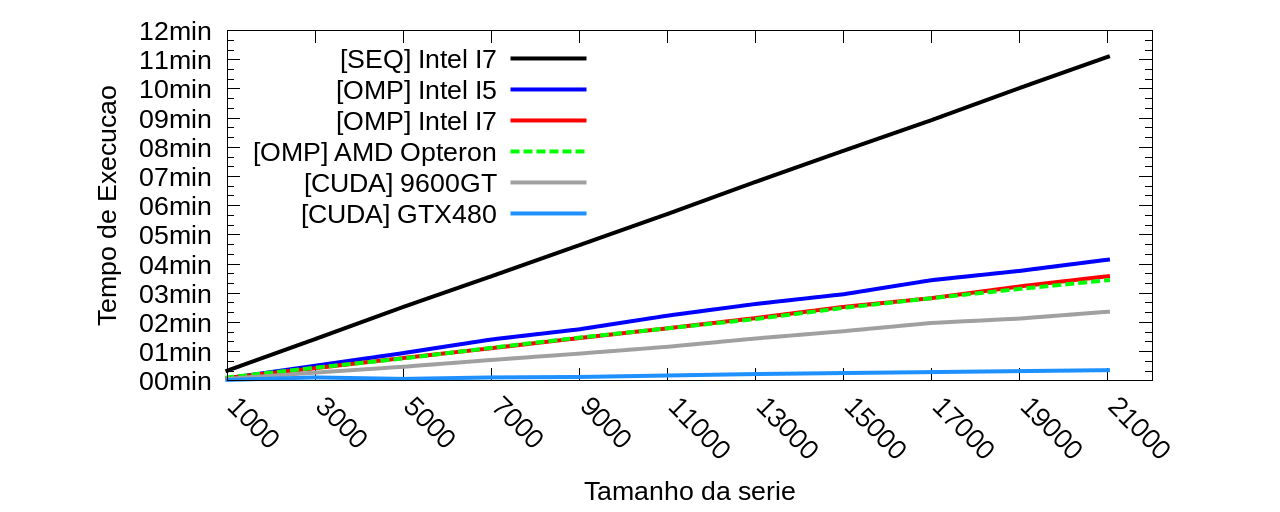
\includegraphics[width=1.0\textwidth]{Imagens/graficos_lanczos/lanczos_tempos.png}
\caption{Gráfico de tempo do algoritmo Filtro de Lanczos}
\label{fig:grafico_tempo_lanczos}
\end{figure}
%%%%%%%%%%%%%%%%%%%%%%%%%%%%%%%%%%%%%%%%%%%%%%%%%%%%%%%%%%

%%%%%%%%%%%%%%%%%%%%%%%%%%%%%%%%%%%%%%%%%%%%%%%%%%%%%%%%%%
% FIGURA
\begin{figure}[H]
\centering
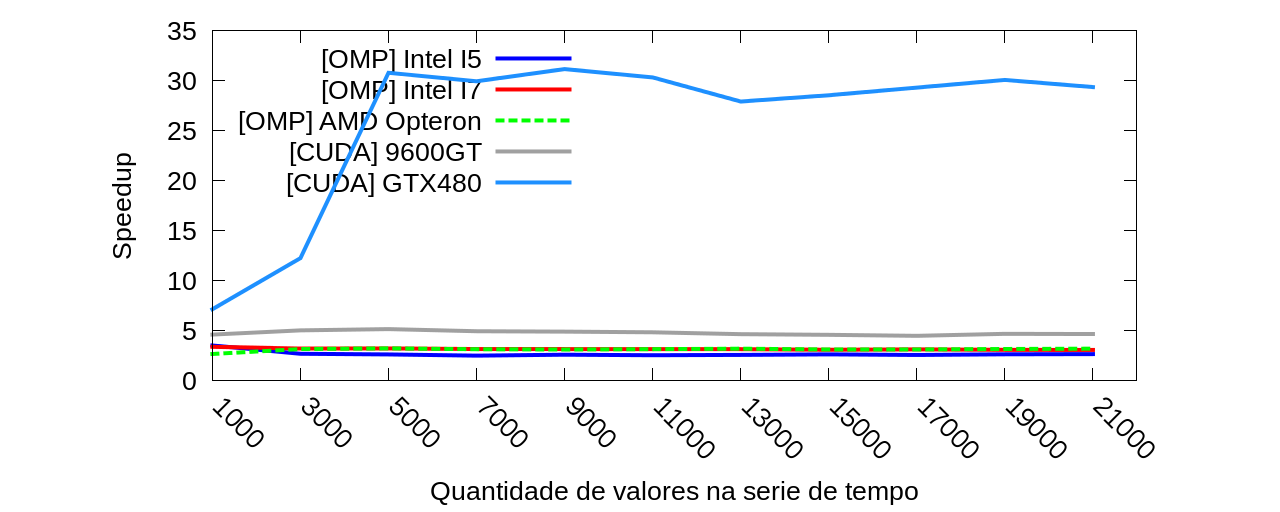
\includegraphics[width=1.0\textwidth]{Imagens/graficos_lanczos/lanczos_speedup.png}
\caption{Gráfico do speedup do algoritmo Filtro de Lanczos}
\label{fig:grafico_speedup_lanczos}
\end{figure}
%%%%%%%%%%%%%%%%%%%%%%%%%%%%%%%%%%%%%%%%%%%%%%%%%%%%%%%%%%

\subsection{Resultados obtidos com o algoritmo Teste de Monte Carlo}

Referencia de \ref{fig:grafico_tempo_mcarlo}

%%%%%%%%%%%%%%%%%%%%%%%%%%%%%%%%%%%%%%%%%%%%%%%%%%%%%%%%%%
% FIGURA
\begin{figure}[H]
\centering
\includegraphics[width=1.0\textwidth]{Imagens/graficos_mcarlo/mcarlo_tempos.png}
\caption{Gráfico de tempo do algoritmo Monte Carlo}
\label{fig:grafico_tempo_mcarlo}
\end{figure}
%%%%%%%%%%%%%%%%%%%%%%%%%%%%%%%%%%%%%%%%%%%%%%%%%%%%%%%%%%

%%%%%%%%%%%%%%%%%%%%%%%%%%%%%%%%%%%%%%%%%%%%%%%%%%%%%%%%%%
% FIGURA
\begin{figure}[H]
\centering
\includegraphics[width=1.0\textwidth]{Imagens/graficos_mcarlo/mcarlo_speedup.png}
\caption{Gráfico do speedup do algoritmo Monte Carlo}
\label{fig:grafico_speedup_mcarlo}
\end{figure}
%%%%%%%%%%%%%%%%%%%%%%%%%%%%%%%%%%%%%%%%%%%%%%%%%%%%%%%%%%

\section{Análise dos resultados}

Como podemos ver, mesmo sem nenhuma otimização tanto no código quanto nos parâmetros de execução do Kernel, os tempos de execução da versão CUDA são significantemente menores, apresentando tempos 6 vezes menores quando usado a GPU 9600GT, e de até 40 vezes com a GPU GTX480 nos testes feitos. Além disso, é perceptível pelas curvas apresentadas no gráfico que essa redução será ainda maior a medida que o tamanho da entrada aumentar, comprovando o poder de processamento das GPUs Nvidia com a tecnologia CUDA.